\documentclass{article}

% -------------------------------------------------
% Packages
% -------------------------------------------------

\usepackage{xcolor}
\usepackage{amsmath}
\usepackage{amssymb}
\usepackage{amsthm}
\usepackage{graphicx}
\usepackage{subcaption}
\usepackage{matlab-prettifier}
\usepackage{listings}
\usepackage{blindtext}
\usepackage{geometry}
\usepackage{float}
\usepackage{dirtytalk}
\usepackage{enumitem}
\usepackage{derivative}
\usepackage{biblatex}
\usepackage{svg}
\usepackage{hyperref}
\usepackage{bbm}
\usepackage{float}
\usepackage{tikz}
\usepackage{pgfplots}
% -------------------------------------------------
% Colors
% -------------------------------------------------

\definecolor{darkgreen}{rgb}{0.0, 0.5, 0.0}

% -------------------------------------------------
% Hyperlinks
% -------------------------------------------------

\hypersetup{
    colorlinks=true,
    linkcolor=blue,
    citecolor=blue,
    urlcolor=blue
}

% -------------------------------------------------
% Theorem environments
% -------------------------------------------------

% Numbered
\newtheorem{theorem}{Theorem}[section]
\newtheorem{lemma}[theorem]{Lemma}
\newtheorem{proposition}[theorem]{Proposition}

% Unnumbered
\newtheorem*{theorem*}{Theorem}
\newtheorem*{lemma*}{Lemma}
\newtheorem*{proposition*}{Proposition}

\theoremstyle{definition}
\newtheorem{definition}[theorem]{Definition}
\newtheorem{example}[theorem]{Example}

\theoremstyle{remark}
\newtheorem{remark}[theorem]{Remark}

% -------------------------------------------------
% Equation numbering
% -------------------------------------------------

% Reset equation numbering at each section
\makeatletter
\@addtoreset{equation}{section}
\makeatother

\renewcommand{\theequation}{\thesection.\arabic{equation}}

% -------------------------------------------------
% Python / MATLAB code formatting
% -------------------------------------------------

\lstset{
    language=Python,
    basicstyle=\ttfamily\small,
    keywordstyle=\color{blue},
    stringstyle=\color{darkgreen},
    commentstyle=\color{gray},
    showstringspaces=false,
    frame=single,
    numbers=left,
    numberstyle=\tiny\color{gray},
    breaklines=true
}

% -------------------------------------------------
% Page geometry
% -------------------------------------------------

\geometry{
    a4paper,
    total={160mm,250mm},
    left=25mm,
    top=30mm,
    footskip=10mm
}

% -------------------------------------------------
% Document settings
% -------------------------------------------------

\setlength{\parindent}{0pt}

% -------------------------------------------------
% Title
% -------------------------------------------------

\title{Monte Carlo Simulation Uge 2}
\author{Thomas Sejer Canham}
\date{\today}

% =================================================
% Document
% =================================================

\begin{document}
\section{Week 1}
\subsection{Likelihood}

We are interested in the likelihood function for a given set of data $y$. This is motivated by the fact that we want to find the parameters $\theta$ that maximize the likelihood of observing the data $y$. The likelihood function is defined as:
\begin{equation}
L(\theta) = f(y ; \theta), \quad \theta \in \Theta.
\end{equation}
This is to be read as the likelihood is a parameterized function of $\theta$ given the data $y$. $\Theta$ is the parameter space, and the the observed data $y$ belongs to the sample space $\mathcal{Y}$. As per usual, when the observed data is independent, the likelihood function can be expressed as the product of the individual likelihoods:
\begin{equation}
L(\theta) = \prod_{i=1}^{n} f(y_i ; \theta), \quad \theta \in \Theta.
\end{equation}
where y is a vector of observed data points $y = (y_1, y_2, \ldots, y_n)$. Sometimes it is more convenient to work with the log-likelihood function, which is defined as:
\begin{equation}
\ell(\theta) = \log L(\theta) = \sum_{i=1}^{n} \log f(y_i ; \theta), \quad \theta \in \Theta.
\end{equation}
From a frequentist perspective, all the information relatated to the parameter $\theta$ is contained in the likelihood function. This is converse to the Bayesian perspective, where we typically have prior information about the parameter or parameter space.


We note that we may observe independent and different quantities $y$ and $z$ that separately carry information about the parameters $\theta$. In such cases, the likelihood function can be expressed as the product of the individual likelihoods:
\begin{equation}
L(  \theta) = L(y; \theta) L(z; \theta), \quad \theta \in \Theta.
\end{equation}
We may find a estimate for $\theta$, to compare it to the maximizing value of the likelihood function, we may define the relative likelihood function as:
\begin{equation}
RL(\theta) = \dfrac{L(\theta)}{\max_{\theta' \in \Theta} L(\theta')}, \quad \theta \in \Theta.
\end{equation}

Finding the maximum likelihood estimate $\hat{\theta}_MLE$ is equivalent to finding the value of $\theta$ that maximizes the likelihood function, or equivalently, the log-likelihood function, as this is a monotonic transformation. Usually, we find the critical points of the likilihood or log-likelihood function by taking the derivative with respect to $\theta$ and setting it equal to zero:
\begin{equation}
 \dfrac{\partial L(\theta)}{\partial \theta} = 0\text{ or }\dfrac{\partial \ell(\theta)}{\partial \theta} = 0.
\end{equation}
However, counter examples do exist:
\begin{example}
    Consider a random sample of size n from a uniform distribution on the interval $[0, \theta]$, where $\theta \leq 0$. The PDF of the uniform distribution is given by:
    \begin{equation}
        f(y; \theta) = \begin{cases}
            \dfrac{1}{\theta} & \text{if } 0 \geq y \geq \theta, \\
            0 & \text{otherwise}.
        \end{cases}
        \end{equation}
    And thus the likelihood function is given by:
\begin{equation}
    L(\theta) = \prod_{i=1}^{n} f(y_i; \theta) \mathbbm{1}(0 \leq y_i \leq \theta) = \dfrac{1}{\theta^n} \mathbbm{1}(\theta \geq \max\{y_1, \ldots, y_n\})
\end{equation}
We see that the likelihood function is a decreasing function of $\theta$ and is only non-zero for values of $\theta$ greater than or equal to the maximum observed value. Therefore, the maximum likelihood estimate is given by $\hat{\theta}_{MLE} = \max\{y_1, \ldots, y_n\}$.
Suppose we have $n = 3$, then visually we will get the plot:
\begin{figure}[H]
    \centering

    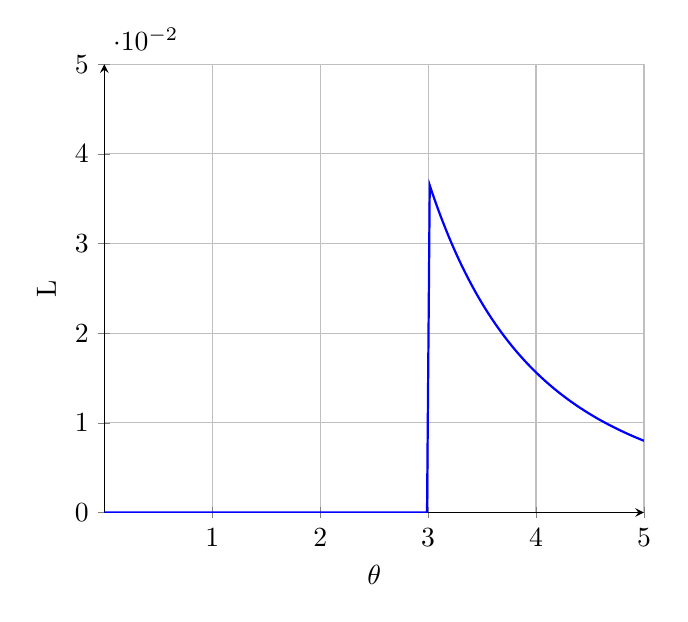
\begin{tikzpicture}
        \begin{axis}[
            axis lines = left,
            xlabel = {$\theta$},
            ylabel = {L},
            ymin = 0,
            ymax = 0.05,
            xmin = 0,
            xmax = 5,
            xtick = {1,2,3,4,5},
            ytick = {0,0.01,0.02,0.03,0.04,0.05},
            grid = major,
            legend pos = north east,
        ]

        \addplot[
            domain = 0:5,
            samples = 200,
            blue,
            thick,
        ]
        {x >= 3 ? 1/x^3 : 0};


        \end{axis}
    \end{tikzpicture}
    \label{fig:likelihood_uniform}
\end{figure}
Evidently, the maximum likelihood is not located at a critical point. Instead, the maximum likelihood is located at the boundary of the parameter space.
$\square$
\end{example}
\subsection{Monotone Transformation of the Data}
The maximum likelihood estimate is invariant under monotone transformations of the data. That is, if we have a monotone transformation $g(y)$ of the data $y$, then the maximum likelihood estimate of $\theta$ based on the transformed data $g(y)$ is the same as the maximum likelihood estimate based on the original data $y$. This property can be useful in practice, as it allows us to work with transformed data that may be easier to analyze or interpret. This follows from (Ute's Notes): \vspace{0.5cm}
Let $h : Y \to Z$ be a bijective function from $Y$ to a new variable $Z = h(Y)$. Then the likelihood function for $\theta$ based on the transformed data $Z$ is given by:
\begin{equation}
    L_Z(\theta) = f_Z(z; \theta) = f_Y(y; \theta) \left| \dfrac{dy}{dz} \right| 
\end{equation}
where $\left| \dfrac{dy}{dz} \right|$ is the Jacobian of $h$. We see that this is independant of $\theta$ and thus the maximum likelihood estimate of $\theta$ is invariant, as location remains unchanged, but the value of the likelihood function may change.

\subsection{Re-parameterization}
We may consider a re-parameterization $\psi = g(\theta)$ where $g$ is a bijective function from the parameter space $\Theta$ to a new parameter space $\Psi$. Then then the following equivalence holds:
\begin{equation}
    L_\Theta(\theta) = L_\Psi(g(\theta)) = L_\Psi(\psi)
\end{equation}
This means that the maximum likelihood estimate of $\hat{\psi} = g(\hat{\theta})$ where $\hat{\theta}$ is the maximum likelihood estimate of $\theta$. This property can be useful in practice, as it allows us to work with re-parameterized models that may be easier to analyze or interpret. \vspace{1em}

Note that the Fisher information is not invariant under re-parameterization. We saw this in Davison excercise 4.3.5,

\subsection{Quadratic Approximation of the Log-Likelihood}
To consider such approximations it is useful to consider some properties of the taylor expansion. The taylor expansion, presented with the first four terms, is given by:
\begin{equation}
f(x) = f(a) + f'(a)(x-a) + \dfrac{f''(a)}{2!}(x-a)^2 + \dfrac{f'''(a)}{3!}(x-a)^3 + R_4
\end{equation}
where $R_4$ is the remainder term. The taylor expansion can be used to approximate a function $f(x)$ around a point $a$. Furthermore, using the Lagrange Remainder theorem, where the approximation is given by:
\begin{equation}
f(x) = f(a) + f'(a)(x-a) + \dfrac{f''(a)}{2!}(x-a)^2 + \dfrac{f'''(c)}{3!}(x-a)^3 + f''''(c)(x-a)^4
\end{equation}
for some $c$ between $a$ and $x$. This is the langrange form of the remainder term, and et guarantees the existence of a point $c$ between $a$ and $x$ such that the remainder is exact. We can use this and the log relative likelihood function to show that the log likelihood is approximately quadratic around the maximum likelihood estimate $\hat{\theta}$. See page 102 of the book.\vspace{1em}

Furthermore, the approximation is useful when considering numerical routines, such as the Newton-Raphson methods for finding the maximum likelihood estimate. Under quadratic assumptions the Newton-Raphson method converges in one step.


\subsection{Sufficient Statistics}
Sometimes we can find the MLE by using a sufficient statistic. The sufficient statistic is some, hopefully lower dimensional, function of the data that contains all the information about the parameter $\theta$. The formal definition is as follows:
\begin{definition}
A statistic $S(y)$ is sufficient for the parameter $\theta$ if the conditional distribution of the data $y$ given the statistic $S(y)$ does not depend on the parameter $\theta$. In other words, once we know the value of the sufficient statistic, we have all the information about $\theta$ that is contained in the data $y$.
\end{definition}
A direct consequence is that the conditional distribution of the data $y$ given the sufficient statistic $S(y)$ is independent of the parameter $\theta$, as such

\begin{equation}
    f_{Y|S}(y|s; \theta) 
\end{equation}
does not depend on $\theta$. This means that the likelihood function can be expressed as a function of the sufficient statistic $S(y)$, and we can use this to find the MLE.

We can also use the factorization theorem to find sufficient statistics. The factorization theorem states that a statistic $S(y)$ is sufficient for the parameter $\theta$ if and only if the likelihood function can be factored into two parts: one that depends on the data $y$ only through the statistic $S(y)$, and another that does not depend on the parameter $\theta$. In other words, we can write the likelihood function as:
\begin{equation}
L(y; \theta) = g(s(y); \theta) h(y)
\end{equation}
where $g$ depends on the data $y$ only through the observed statistic $s(y)$ and $h$ does not depend on the parameter $\theta$.

\subsection{Information}
The observed information is defined as the negative of the second derivative of the log-likelihood function with respect to the parameter $\theta$:
\begin{equation}
    J(\theta) = -\dfrac{\partial^2 \ell(\theta)}{\partial \theta^2}
\end{equation}
We have a lot of observered information, when this curvature is large, that is, the log-likelihood function is steep around the maximum likelihood estimate, and low observed information when the curvature is small, that is, the log-likelihood function is flat around the maximum likelihood estimate. Note that we can only speak of large or small curvature in relation to the curvature of the log-likelihood function at other values of $\theta$. This motivates the use of relative likelihood. \vspace{0.5cm}

Before we conduct an experiment, we can use the Fisher information to quantify the amount of information that we expect to gain about the parameter $\theta$ from the experiment. The Fisher information is defined as the expected value of the observed information:
\begin{equation}
    I(\theta) = \mathbb{E}[J(\theta)] = -\mathbb{E}\left[\dfrac{\partial^2 \ell(\theta)}{\partial \theta^2}\right]  
\end{equation}
To find the Fisher information in practice, we can replace the yet to be observed data $y$ with the corresponding random variable $Y$ and take the expectation with respect to the distribution of $Y$. 

\subsection{Relative Efficiency}
Assume that we have two distributions A and B, that contain information about the same parameter $\theta$. We can compare the efficiency of the two distributions by comparing their Fisher information. This gives us ground for model selection, as we might be able to choose a model with more or the same information, but with less complexity or work involved. The relative efficiency of distribution A with respect to distribution B is defined as:
\begin{equation}
    \dfrac{I_A(\theta)}{I_B(\theta)}
\end{equation}
Recall that $i_X(\theta)$ is the Fisher information of a single sample from distribution X. Sampling schemes are said to be equally efficient if
\begin{equation}
    \dfrac{i_A(\theta)}{i_B(\theta)} = \dfrac{n_B}{n_A}.
\end{equation}
If we rewrite this as
\begin{equation}
    n_B = \dfrac{i_A(\theta)}{i_B(\theta)} n_A,
\end{equation}
we see that this shows how many samples from distribution B we need to get the same amount of information as $n_A$ samples from distribution A.

\section{Week 2}

In week 2 we worked with stochastic convergence, the consistency and asymptotic normality of the maximum likelihood estimator, and the Kullback-Leibler divergence.

\subsection{Stochastic Convergence}
Stochastic convergence is a fundamental concept in probability theory and statistics. It describes the behavior of a sequence of random variables as the number of observations increases. Note that a sequence is NOT a sample, but rather a fixed behavior of a random variable as the number of observations increases. 

\subsubsection{Example of a Sequence}
And example of a sequence is the sample mean of a random variable $X$ with finite mean $\mu$ and variance $\sigma^2$. The sample mean is defined as:
\begin{equation}
    \bar{X}_n = \dfrac{1}{n} \sum_{i=1}^{n} X_i
\end{equation}
So for $n = 1$ we have
\begin{equation}
    \bar{X}_1 = X_1
\end{equation}
and for $n = 2$ we have
\begin{equation}
    \bar{X}_2 = \dfrac{1}{2} (X_1 + X_2)
\end{equation}
And so on. Thus the sequence of sample means is given by:
\begin{equation}
    \{\bar{X}_n\}_{n=1}^{\infty} = \{\bar{X}_1, \bar{X}_2, \bar{X}_3, \ldots\}
\end{equation}

\subsection{Modes of Convergence}
We have seen three different modes of convergence: almost sure convergence, convergence in probability, and convergence in distribution. We will define each of these modes of convergence and discuss their properties.

\subsubsection{Almost Sure Convergence}
A sequence of random variables $\{X_n\}_{n=1}^{\infty}$ converges almost surely to a random variable $X$ if:
\begin{equation}
    P\left(\lim_{n \to \infty} X_n = X\right) = 1
\end{equation}
Intuitively, this means that the behavior of the sequence of random variables, will asymptotically match the behavior of the random variable $X$ with probability 1. An example is a sequence $X_n$ on the sample space $\Omega$ such that $X_n(\omega) = \mathbbm{1}(0\leq \omega \leq \dfrac{n+1}{2n})$ if we then let 
$$
A = \{\omega \in \Omega : \lim_{n \to \infty} X_n(\omega) = X(\omega)\}
$$
where $X(\omega) = \mathbbm{1}(0\leq \omega < \frac{1}{2})$ Then we have to prove that $P(\omega \in A) = 1$. Breifly, we can see that for $\omega < \frac{1}{2}$, $X_n(\omega) = 1$ for all $n$, and for $\omega > \frac{1}{2}$, $X_n(\omega) = 0$ for all $n$. Thus, the only point of concern is $\omega = \frac{1}{2}$, but this is a single point and has probability 0. Therefore, we have that $P(A) = 1$ and thus $X_n \to X$ almost surely. If we have almost sure convergence, then we also have convergence in probability, but the converse is not true, so
$$X_n \xrightarrow[]{a.s} X \implies X_n \xrightarrow[]{P} X$$
Most notably, we have the strong law of large numbers, which states that the sample mean converges almost surely to the population mean.
\begin{equation}
    \bar{X}_n = \dfrac{1}{n} \sum_{i=1}^{n} X_i \xrightarrow[]{a.s} \mu
\end{equation}

\subsubsection{Convergence in Probability}
A sequence of random variables $\{X_n\}_{n=1}^{\infty}$ converges in probability to a random variable $X$ if:
\begin{equation}
    P\left(\left|X_n - X\right| > \epsilon\right) \to 0 \quad \text{as } n \to \infty
\end{equation}
for every $\epsilon > 0$. This means that the probability that the difference between $X_n$ and $X$ is greater than any positive number $\epsilon$ goes to zero as the number of observations increases. An example is the convergence in probability of the exponential distribution to the degenerate 0 distribution. Let $X_n \sim \text{Exp}(n)$, then we have that
\begin{equation}
    P\left(\left|X_n - 0\right| > \epsilon\right) = P(X_n > \epsilon) = e^{-n\epsilon} \to 0 \quad \text{as } n \to \infty
\end{equation}
Most notably, we have the weak law of large numbers, which states that the sample mean converges in probability to the population mean. 
\begin{equation}
    \bar{X}_n = \dfrac{1}{n} \sum_{i=1}^{n} X_i \xrightarrow[]{P} \mu
\end{equation}

\subsubsection{Convergence in Distribution}
A sequence of random variables $\{X_n\}_{n=1}^{\infty}$ converges in distribution to a random variable $X$ if:
\begin{equation}
    F_{X_n}(x) \to F_X(x) \quad \text{as } n \to \infty
\end{equation}
for all points $x$ where $F_X(x)$ is continuous. Here, $F_{X_n}(x)$ and $F_X(x)$ are the cumulative distribution functions of $X_n$ and $X$, respectively.

\subsection{Slutsky's Lemma}
This lemma desribes the relation between modes of convergence, let $S_n$ and $U_n$ be sequences of random variables and $S$ and $U$ be random variables and let $s_0$ and $u_0$ be constants. Then we have the following results:
\begin{lemma}[Slutsky's Lemma]
    \begin{equation}
        S_n \xrightarrow[]{P} S \implies S_n \xrightarrow{D} S
    \end{equation}
    \begin{equation}
        S_n \xrightarrow[]{D} s_0 \implies S_n \xrightarrow{P} s_0
    \end{equation}
    \begin{equation}
        S_n \xrightarrow[]{D} S,\, U_n \xrightarrow[]{P} u_0 \implies S_n + U_n \xrightarrow{D} S + u_0, \,S_n U_n \xrightarrow{D} S u_0
    \end{equation}
    \end{lemma}
Note that $S= s_0$ and $U = u_0$ are also valid (degenerate) random variables, thus
$$S_n \xrightarrow{P} s_0 \iff S_n \xrightarrow{D} s_0$$

\subsection{Kullback-Leibler disrepancy and the Convegence of the MLE}

We can use Jensen's inequality to shot that the Kullback-Leibler discrepancy $D(f_\theta, f_{\theta_0}) \geq 0$. The difference of the mean-log-likelihoods converges almost surely to the negative Kullback-Leibler discrepancy, and thus the difference of the log-likelihoods
$$\ell(\theta) - \ell(\theta_0) \xrightarrow[]{D} -nD(f_\theta, f_{\theta_0}) \to -infty$$ for $n \to \infty$.
This mean for any $\delta >0$, there exists a local region around $\theta_0$ such that for any sequence of random variables $Y_n$ there exists a $N$ such that for all $n > N$, there is a interval where $-D(f_{\theta_0-\delta}$ and $-D(f_{\theta_0+\delta})$ are negative, and thus the maximum likelihood will lie in this interval with probability 1. This shows that the maximum likelihood estimator is consistent, that is, it converges in probability to the true parameter value $\theta_0$ as the sample size $n$ increases.

To summarize, we use the Kullback-Leibler discrepancy to prove that the estimator will be squeezed into a local region around the true parameter value $\theta_0$, where values of $\theta$ that are not the true parameter value will have a lower likelihood, and thus the maximum likelihood estimator will converge to the true parameter value as the sample size increases.
\end{document}